\section{Durchführung}
\label{sec:Durchführung}
\begin{figure}[H]
    \centering
    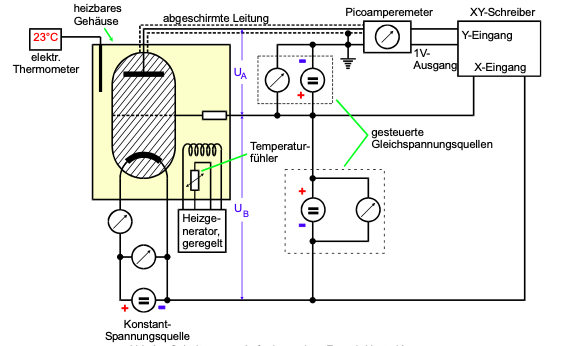
\includegraphics[width=0.7\textwidth]{content/Bilder/Aufbau.png}
    \caption{Schaltbild zur Aufnahme einer Franck-Hertz-Kurve Q\cite{anleitungV601}.}
    \label{fig:Aufbau}
\end{figure}
Für beide Durchführungen wird der Versuchaufbau in Abbildung \ref{fig:Aufbau} verwendet.

\subsection{Integrale Energieverteilung der beschleunigten Elektronen}
Im ersten Teil der Durchführung wird die integrale Energieverteilung der beschleunigten Elektronen bestimmt. 
Hierfür wird der Auffängerstrom $I_{\text{A}}$ in Abhängigkeit von der Bremsspannung $U_{\text{A}}$ gemessen, welche 
mithilfe des XY-Schreibers aufgezeichnet werden. 
Dabei wird die Beschleunigerspannung auf $U_{\text{B}} = 11\,\unit{\volt}$ eingestellt und wird nicht weiter verändert. 
Diese Messungen werden bei Zimmertemperatur und für eine Temperatur zwischen $T = 140-160\,\unit{\celsius}$ durchgeführt.

\subsection{Franck-Hertz-Kurven}
Beim zweiten Teil des Versuchs werden je eine Franck-Hertz-Kurven für drei verschiedene Temperaturen mithilfe des XY-Schreibers aufgenommen. 
Hier werden der Auffängerstrom $I_{\text{A}}$ in Abhängigkeit der Beschleungierspannung $U_{\text{B}}$, im Bereich von 
$0 < U_{\text{B}} < 60\,\unit{\volt}$, gemessen. Währenddessen bleib die Bremsspannung konstant bei $U_{\text{A}}= 1\,\unit{\volt}$.
Für die Auswertung wird anschließend die Kurve ausgewählt, bei der die Maxima und Minima besonders gut ausgeprägt sind. 